\documentclass[a4paper, 12pt]{report}
\usepackage[utf8]{inputenc}
\usepackage[T1]{fontenc}

\usepackage{xcolor}
\usepackage{afterpage}

\usepackage{relsize}
\usepackage{moresize}

\usepackage{graphicx}
\usepackage{geometry}

% [CHANGE] The title of your thesis. If your thesis has a subtitle, then this
% should appear right below the main title, in a smaller font.
\newcommand{\theTitle}{Quadratic Forms in \\
\vspace{0.5em}
Convolutional Neural Networks}
\newcommand{\theSubTitle}{}


% [CHANGE] Your full name. In case of multiple names, you can include their
% initials as well, e.g. "Robin G.J. van Achteren".
\newcommand{\theAuthor}{Peter Adema}

% [CHANGE] Your student ID, as this has been assigned to you by the UvA
% administration.
\newcommand{\theStudentID}{14460165}

% [CHANGE] The name of your supervisor(s). Include the titles of your supervisor(s),
% as well as the initials for *all* of his/her first names.
\newcommand{\theSupervisor}{Dr.\ ir.\ R.\ van den Boomgaard} % Dr. Ing. L. Dorst

% [CHANGE] The address of the institute at which your supervisor is working.
% Be sure to include (1) institute (is appropriate), (2) faculty (if
% appropriate), (3) organisation name, (4) organisation address (2 lines).
\newcommand{\theInstitute}{
Informatics Institute \\ %Institute for Logic, Language and Computation
Faculty of Science\\
University of Amsterdam\\
Science Park 900 \\ 
1098 XH Amsterdam 
}

% [CHANGE] The semester in which you started your thesis.
\newcommand{\theDate}{Semester 2, 2024-2025}



\usepackage[shortlabels]{enumitem}
\usepackage{graphicx}

\usepackage{hyperref}
\usepackage{amsmath}
\usepackage{amssymb}
\usepackage{amsthm}
\usepackage{mathabx}
%\usepackage{apacite}
\usepackage{caption}
\usepackage{listings}
\usepackage{xcolor}
\def\comment#1{\color{red}#1\color{black}}
\usepackage{bbold}
\DeclareMathOperator{\boxclose}{\vcenter{\hbox{$\blacksquare$}}}
\DeclareMathOperator{\boxopen}{\Box}


\begin{document}
\pagestyle{empty}
\begin{center}

\vspace{2.5cm}


\begin{Huge}
% see definition at beginning of document
\theTitle
\end{Huge} \\

\vspace{0.5 cm}

\begin{Large}
\theSubTitle
\end{Large}

\vspace{1.5cm}

% see definition at beginning of document
\theAuthor\\
% see definition at beginning of document
\theStudentID

\vspace{1.5cm}

% [DO NOT CHANGE]
Bachelor thesis\\
Credits: 18 EC

\vspace{0.5cm}

% [DO NOT CHANGE] The name of the educational programme.
Bachelor \textit{Kunstmatige Intelligentie} \\
\vspace{0.25cm}

\includegraphics[width=0.075\paperwidth]{figures/uva_logo} \\
\vspace{0.1cm}

% [DO NOT CHANGE] The address of the educational programme.
University of Amsterdam\\
Faculty of Science\\
Science Park 900\\
1098 XH Amsterdam

\vspace{2cm}

\emph{Supervisor}\\

% see definition at beginning of document
\theSupervisor

\vspace{0.25cm}

% see definition at beginning of document
\theInstitute

\vspace{1.0cm}

% see definition at beginning of document
\theDate

\end{center}
\newpage



\pagenumbering{arabic}
\setcounter{page}{1}
\pagestyle{plain} 

\newgeometry{a4paper, textwidth=400.0pt, textheight=740.0pt}
\chapter{Introduction}
In the field of computer vision, machine learning has been successfully applied for societal benefit in various ways, ranging from analysing medical imaging data \cite{esteva2021deep, jain2015computer} to classifying agricultural produce \cite{wan2020faster, sivaranjani2022overview} and recognising license plate numbers \cite{xie2018new}. One of the primary tools used in these applications is the Convolutional Neural Network (CNN) \cite{le1990handwritten}, a type of neural network that leverages existing theoretical knowledge of image processing to learn representations of images more efficiently.

Two components are often seen within a typical CNN: the titular convolutional layer, which analyses the image, and a pooling layer, which compresses the image representation (see \cite{introconvnets} for an introduction). The latter pooling layer is often implemented as a max-pooling layer, which selects the highest value in a small area around every point in the image. Slightly more generally, a max-pooling layer can be seen as an operation that weighs neighbours around a point in the image and selects the neighbour with the highest weight, but with all neighbours being weighed equally. However, this general perspective suggests the possibility of a variation on a max-pooling layer where pixels are not weighed equally: perhaps pixels further away from the centre are considered less in the selection for the maximum.

This idea has been formalised in mathematical morphology as dilation \cite{heijmans1996morphological} and in tropical geometry as a max-plus convolution \cite{maragos}. Using this formalism, a separate function $G$ (the structuring element or kernel) defines the weighting for neighbouring pixels. This function can be parameterised in various ways, but a concave function centred around the origin is typically used for G. One such function is the quadratic function $f(x)=x^T\Sigma^{-1}x$, and another is its isotropic form $f(x)=x^T(sI)^{-1}x$, with parameters $\Sigma$ and $s$ respectively \cite{Boomgaard1999NumericalSS}.

Previous studies \cite{groenendijk2022morphpool} and theses \cite{thierrybsc, koenbsc} have investigated the possibility of using such a dilation (generalised max-pooling) with an isotropic quadratic structuring element as a layer within a CNN, with the parameter $s$ being learned via gradient descent (a standard optimisation method within machine learning). These previous works showed that using an isotropic quadratic kernel (which is strictly more expressive than a standard max-pooling) resulted in higher performance on a small selection of datasets. This thesis aims to expand upon this by examining using an anisotropic quadratic structuring element within the dilation, specifically whether the anisotropic parameters $\Sigma$ could also be learned via gradient descent. The expectation would be that since anisotropic quadratic kernels are again strictly more expressive than the isotropic versions, such a dilation layer would further improve performance.

\newpage
\section{Related work}
\comment{For now, I've just copied my literature survey from the project proposal.\\ I intend to rewrite this evenutally, though: no need to review this for now.}

Modern Convolutional Neural Networks (CNNs) often use linear convolutional layers to process images and max-pooling layers to condense information and shrink the feature space \cite{introconvnets}. However, both of these operations are equivalent to a semifield convolution: the first in the linear field (with a learned kernel) and the second in the tropical-max field (with a step-function-like kernel) \cite{bellaardaxiomatic}. In \cite{bellaardaxiomatic}, Bellaard et al. provide an axiomatic foundation for using various semifields within the context of PDE-CNNs but do not discuss using semifields for conventional (discrete) CNNs. 

The ideas underlying the usage of tropical fields are, however, older than \cite{bellaardaxiomatic}: the field of mathematical morphology researches the shapes and forms of objects and functions, and two of the core operators within mathematical morphology are dilation (equivalent to a tropical-max correlation) and erosion (equivalent to a tropical-min correlation) \cite{maragos}. Heijmans \cite{heijmans1996morphological} is an excellent treatment of many of the theoretical fundaments and generalised cases of morphology, with Chapter 11 describing morphology for grey-scale images (most similar to the convolutional operations relevant to this project). Furthermore, morphological operations with specifically a quadratic structuring element were researched by Boomgaard in \cite{Boomgaard1999NumericalSS} and other papers, showing that many aspects of the resulting calculation can be performed in closed form without first approximating the quadratic into a fixed-size kernel.

Another paper of note regarding the efficient calculation of the convolutional stencil in tropical semifields may be \cite{fastanifilter}, in which Geusebroak and van de Weijer discuss how to perform an efficient calculation for the linear field with a Gaussian kernel. Whether such methods will be needed within this project is yet unclear, but the notes regarding approximate separability by reorienting the axes of a quadratic show a possible direction for further performance improvements.

Besides relevant theory, there are also some more recent pieces of literature somewhat close to this topic. Notably, \cite{qlin1, qlin2} show that a CNN that learns quadratic scale parameters for the kernels of its linear convolution can, in some cases, learn to perform tasks similar to those of a CNN that directly learns all kernel parameters. This adjustment significantly reduces the parameters required for the linear convolutions replaced in such a way. Furthermore, it is equivalent to the original Bachelor project proposal, where the task would have been to parameterise a linear convolution with the PDF of a Gaussian. 

Finally, previous projects under Dr. Boomgaard have partly investigated discrete subfield convolutions. The isotropic case (where scales are uncorrelated and bound between dimensions) for tropical-max fields has been relatively well-researched by \cite{thierrybsc, koenbsc}, showing minor performance increases in basic vision models. However, a more general treatment of anisotropic kernels in tropical max semifields (and other fields) is not yet present within either the public domain or the UvA collection of theses. 

\chapter{Background}
First, mathematical formalisms must be covered to understand the concepts discussed in later sections. These include the convolutional operator, its generalisation using semifields, and relevant semifields from mathematical morphology. Subsequently, we will discuss variations on the convolutional operator, as well as quadratic distance functions and a method for learning the positive definite matrices parameterising them.

\section{Convolutional operator}
At the core of a convolutional neural network is the convolutional operation $f*g$. The general form of a continuous convolution of functions $f$ and $g$ can be written as:
\begin{align}
(f*g)(x) &= \int_{y\in\mathcal{D}} f(x-y)\; g(y)	,
\end{align}
where $\mathcal{D}$ is the (continuous) domain of $f$ and $g$. However, save for a handful of functions whose convolutions can be calculated algebraically, we are typically required to approximate this convolution in the discrete domain. In this case, we approximate the functions $f$ and $g$ by sampling them at fixed intervals, the result of which can be represented as discrete arrays $F$ and $G$. A discrete convolution could then be written as \cite{szeliski2022computer}:
\begin{align}
(F*G)[x] &= \sum_{y\in\mathcal{I}} F[x-y]\; G[y],
\end{align}
where $\mathcal{I}$ is the set of all indices in the domain of $F$ and $G$ (e.g. $\mathcal{I}=\mathbb{Z}^2$ for infinitely large 2D images and kernels), and $G$ is typically referred to as the (convolutional) kernel.


\section{Fields and semifield convolutions}
In the convolutional operator, a part of the image is repeatedly multiplied element-wise with a kernel, and the resulting values are summed to obtain an activation for each point. However, while we typically use scalar addition and multiplication in this calculation, it is also possible to use different operators in the reduction by defining a different field in which the reduction is done. In this section, we will briefly look at the concept of fields insofar as they are relevant to implementing an alternative version of the convolutional operator.

In mathematics, a field is a set of values with a pair of operators that work on those values: one operator corresponds to the concept of addition, and one operator corresponds to the concept of multiplication. Fields are, in effect, a generalisation of standard addition and multiplication on integers or reals that allow for describing a set of values other than typical scalars or an alternate method for combining typical numbers. Formally, a field can be described as a tuple $(\mathcal{F}, \oplus, \otimes)$, where the operators $\oplus$ and $\otimes$ are of the type $\mathcal{F}\times\mathcal{F}\rightarrow\mathcal{F}$. Furthermore, the operators $\oplus$ and $\otimes$ are both beholden to the field axioms: informally, a set of rules to ensure they act 'similarly' to standard scalar addition and multiplication. 

These field axioms can be written as (adapted from \cite{beachy2006abstract}, page 120):
\begin{align}
\textrm{$\oplus$ is associative: }&\forall a,b,c\in \mathcal{F} &  a \oplus (b \oplus c) = (a\oplus b) \oplus c \\ 
\textrm{$\otimes$ is associative: }&\forall a,b,c\in \mathcal{F} &  a \otimes (b \otimes c) = (a\otimes b) \otimes c \\ 
\textrm{$\oplus$ is commutative: }&\forall a,b\in \mathcal{F} & a\oplus b = a  \oplus a \\
\textrm{$\otimes$ is commutative: }&\forall a,b\in \mathcal{F} & a\otimes b = a  \otimes a \\
\oplus\textrm{ has an identity: }& \exists \mathbb{0} ~\forall a\in \mathcal{F} & a\oplus \mathbb{0} = a \\ 
\otimes\textrm{ has an identity: }& \exists \mathbb{1} ~\forall a\in \mathcal{F} & a\otimes \mathbb{1} = a \\ 
\oplus\textrm{ has inverse elements: }& \forall a~\exists b\in \mathcal{F} & a\oplus b = \mathbb{0} \label{eq:additive-inverse}  \\ 
\otimes\textrm{ has inverse elements: }& \forall a~\exists b\in \mathcal{F} & a\otimes b = \mathbb{1}  \\ 
\otimes \textrm{ distributes over $\oplus$: }&\forall a,b,c\in \mathcal{F} & a\otimes (b \oplus c) = (a\otimes b)\oplus(a\otimes c)
\end{align}

One use case for fields in machine learning is to describe a weighted reduction (as in a kernel-based convolution) more generally. To better understand this, let us return to the example of the convolutional operator. In this case, we must reduce the neighbourhood around a pixel $x$ in the image $F$, weighted by the values in the kernel $G$. While this would typically be written as:
\begin{align}
	(F*G)[x] &= \sum_{y\in\mathcal{I}} F[x-y]\; G[y],
\end{align}

\noindent
we could instead use a field $L=(\mathcal{F}, \oplus, \otimes)$ and write a similar operation:

\begin{align}
	(F ~\textcircled{$*$}_L\; G)[x] &=\bigoplus_{y\in \mathcal{I}} F[x-y] \otimes G[y] \label{eq:semifield-conv}
\end{align}
\noindent
Performing this operation does not, strictly speaking, require any of the above field axioms to hold for $\oplus$ or $\otimes$: the only relevant restriction would be that of the types being $\mathcal{F}\times\mathcal{F}\rightarrow\mathcal{F}$. Implementing this operation for a CNN would further require both operators to be differentiable, and for $\mathbb{0}$ to exist (to deal with border effects in a convolution). However, it is generally also useful for the reduction operator $\oplus$ to be both associative and commutative, as this makes the order of elements in the input irrelevant, promoting the stability of the result and allowing efficient parallel implementation of the reduction \cite{ppad}. Furthermore, most of the field axioms hold regardless for most operators we wish to use for $\oplus$ and $\otimes$. As such, we will use a semifield \cite{bellaardaxiomatic}:\\
\textbf{
A semifield is a field, except an additive ($\oplus$) inverse (Eq. \ref{eq:additive-inverse}) does not necessarily exist.
}

We can then define the operator $\textcircled{$*$}_L$ for the following sections (identically to Eq. \ref{eq:semifield-conv}) as the semifield convolutional operator for any semifield $L$.

\section{Semifields from mathematical morphology}
Knowing that an operator similar to convolution can be used in any semifield, we can examine if there are relevant semifields in which we can perform a convolution other than the standard linear field. For this, we can take inspiration from mathematical morphology, the study of object and function shapes.

Two core classes of discrete operators from mathematical morphology are dilations and erosions, where dilations informally correspond with 'making a function larger' (scaling the umbra of a function), and erosions with 'making a function smaller'. The result of the common dilation is shown in Fig. \ref{fig:dil-illust}. Examining the local effects of the dilation more closely, we can see that it is somewhat similar to taking a local maximum, which can also be seen in the formula for this dilation operator $\boxplus$  (from \cite{heijmans1996morphological}, using the Minkowski sum): 
\begin{align}
F \boxplus G \textrm{, where }(F \boxplus G)[x] = \bigvee_ {y\in\mathcal{I}} \left(F[x-y] + G[y]\right)	
\end{align}
\noindent
Here, $F$ is the image (or object or sampled function) to be dilated, $G$ is a structuring element describing how the dilation will occur, and $\bigvee$ denotes the supremum. If we further restrict $F$ and $G$ to be of finite size, then $\mathcal{I}$ will be of finite size, and the correspondence with the local maximum becomes exact:
\begin{align}
\textrm{For finite-size }F\textrm{ and }G: (F \boxplus G)[x] = \max_ {y\in\mathcal{I}} \left(F[x-y] + G[y]\right)	
\end{align}
 An intuitive explanation would be to see the structuring element $G$ as a (negated) distance function and the dilation $\boxplus$ as the operation that takes the highest value weighted by how 'close' it is to $x$. If $G$ is a step function with value zero near its centre and $-\infty$ outside (Fig. \ref{fig:dil-illust}, first row), we can see that this is precisely taking the maximum value in the area where $G$ is zero. However, we may also wish to use a quadratic (Fig. \ref{fig:dil-illust}, second row) or other function as $G$. Depending on $G$, we may still be able to perform the dilation exactly (using algebraic solutions and/or leveraging separability), but to compute the dilation in the general case, we may wish to clip $G$ to be above $-\infty$ in only a constrained domain (Fig. \ref{fig:dil-illust}, third row). The dilation with the clipped version of $F\boxplus G_{clipped}$ could then be seen as an approximation of the dilation $F\boxplus G$ with the full (unclipped) $G$ while having the advantage that the set of relevant indices $\mathcal{I}$ is bounded in size. It should be noted, however, that if $F$ is $K$-Lipschitz and $G$ is strictly decreasing with the second derivative $|\delta^2 G|>K$ outside a central area, then clipping $G$ to this central area will not change the result of the dilation ($F\boxplus G_{clipped}$ is then exact, see Appendix \ref{sec:lipschitz}).

Looking at the operation performed by dilation more closely, we can see that it is, in effect, a maximum operation weighted by a distance function. Similarities with the weighted reduction in the semifield convolution $\textcircled{$*$}_L$ may lead us to believe that this can also be viewed as a convolution in the appropriate semifield $L$, and this is indeed the case. By defining $\oplus=\max$ and $\otimes=+$, we obtain the tropical max semifield $T_+=(\mathbb{R}\cup\{-\infty\},\max,+)$ with neutral elements $(\mathbb{0}=-\infty, \mathbb{1}=0)$ \cite{maragos, bellaardaxiomatic}. A convolution $F \;\textcircled{$*$}_{T_+} G$ in this tropical semifield $T_+$ (also known as a max-plus convolution \cite{maragos}) would then be $\boxplus$:
\begin{align*}
	(F ~\textcircled{$*$}_{T_+} G)[x]
	&= \bigoplus_{y\in \mathcal{I}}F[x-y] \otimes G[y] \\
	&= \max_{y\in \mathcal{I}}\left(F[x-y] + G[y]\right) \\
	&= (F \boxplus G)[x]
\end{align*}

\begin{figure}[h!]
  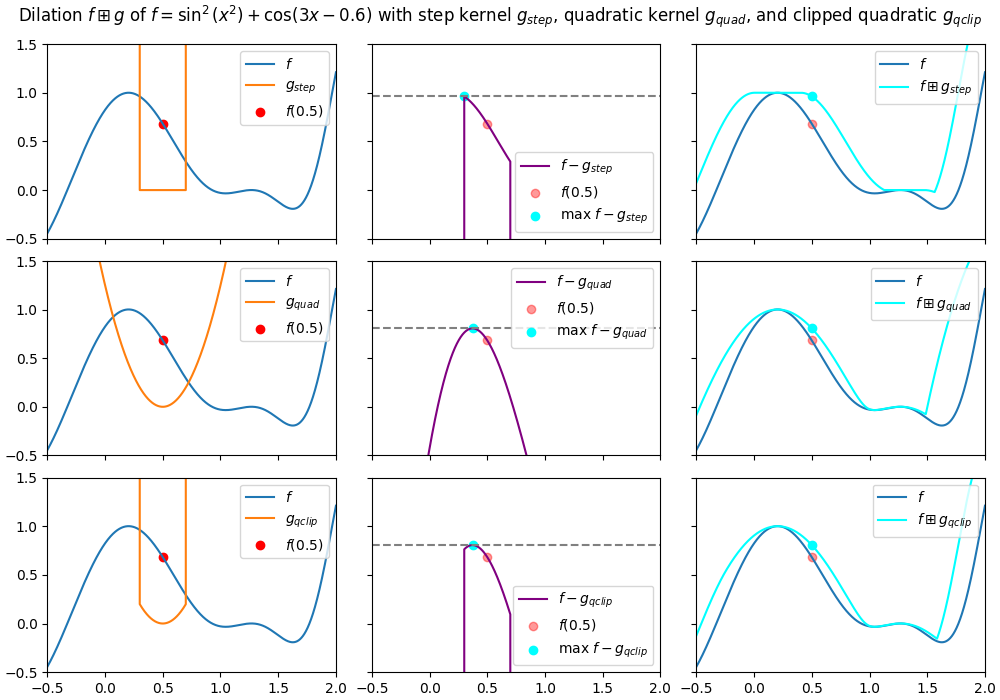
\includegraphics[width=\textwidth]{figures/dilation_illustration.png}
  \caption{Illustration of the effects of the dilation $\boxplus$ with three kernels on a sinusoidal $f$. $g_{step}=0$ in a region of size 0.5 and $-\infty$ outside, while $g_{quad}=-5x^2$ and $g_{qclip}=g_{quad}+g_{step}$. An alternative intuition for $\boxplus$ is also illustrated, corresponding with 'lowering' a negated version of $g'$ down towards the point $x$ until it intersects $f$ and taking the value of the lowered and flipped $g'(x)$ as the result of $\boxplus$ at point $x$. Note the continuous, thus lowercase $f$ and $g$.}
  \label{fig:dil-illust}
\end{figure}
\noindent
This result is interesting because we can see the standard max pooling layer in a convolutional neural network as a dilation with a fixed, step-function-like $G$ (a 2D version of $G_{step}$ from Fig. \ref{fig:dil-illust}). Generalising $G$ to be a quadratic form is a logical next step, where this thesis focuses on the anisotropic case.

In mathematical morphology, dilations and erosions come in pairs named adjunctions. It can be shown that the erosion which adjoins $\boxplus$ (henceforth referred to as the operator $\boxminus$) is effectively a minimum (infimum in the infinite case) weighted by a (negated) distance function \cite{heijmans1996morphological}: 
\begin{align}
	(F \boxminus G)[x]=\min_{y\in \mathcal{I}}(F[x+y] - G[y])
\end{align}
\noindent
Using similar logic as above, we can show that, in the corresponding tropical min semifield $T_-=(\mathbb{R}\cup\{\infty\},\min,+)$\footnote{For both $T_+$ and $T_-$, it should be noted that standard addition $+$ is undefined for $\pm\infty$. In accordance with \cite{maragos}, we define $\forall x: x+(-\infty)=(-\infty)$ in $T_+$, while $\forall x: x+\infty=\infty$ in $T_-$} \cite{maragos} with neutral elements $(\mathbb{0}=\infty, \mathbb{1}=0)$, the convolution with $\check{G}^*(x)=-G(-x)$ is equivalent to the erosion $\boxminus$:
\begin{align}
	(F ~\textcircled{$*$}~ \check{G}^*(x))[x]
	&= \bigoplus_{y\in \mathcal{I}}F[x-y] \otimes \check{G}^*(x)[y] \\
	&= \min{y\in \mathcal{I}}(F[x-y] + \check{G}^*(x)[y]) \\
	&= \min{y\in \mathcal{I}}(F[x-y] - G[-y]) \\
	&= \min{y^*\in \mathcal{I}}(F[x+y^*] - G[y^*]) \\
	&= (F \boxminus G)[x]
\end{align}

\section{Further relevant mathematical morphology}
Besides the common adjoint $(\boxplus,\; \boxminus)$ using $+$ and $-$ as the operators weighing each point, one can also define an adjoint that uses multiplication and division. This alternate adjoint on $\mathbb{R}_+$ then has the dilation $\dot \boxplus$, defined as \cite{heijmans1996morphological}:
\begin{align}
	(F~ \dot\boxplus~ G)[x] &= \bigvee_{y\in \mathcal{I}}F[x-y]G[y]
\end{align}
However, it can be shown that this adjoint is equivalent (anamorphic) to the common adjoint $(\boxplus,\; \boxminus)$ using the transformation $t(x)=e^x$ and its inverse $t^{-1}(x)=\log(x)$. As such, using $\dot \boxplus$ would not result in a more expressive convolution while complicating implementation with the requirement of $\mathbb{R}_+$.

Two other concepts from mathematical morphology that do increase expressivity are the concepts of openings and closings \cite{heijmans1996morphological, gonzalez2017}. Here, an opening is an operator using an adjoint, where the input is first eroded and then dilated with the same structuring element $G$. Notably, an opening is anti-extensive (decreasing), meaning that for $(\boxplus,\; \boxminus)$ we can write the opening $\boxopen$:
\begin{align}
	\forall x\in\mathcal{I}~~(F ~\boxopen~ G)[x] &= ((F\;\boxminus\; G)\;\boxplus\;G)[x] \leq F[x]
\intertext{
The operator dual to an opening is the closing using the same adjoint: here, a closing refers to first performing a dilation, and then performing the adjoining erosion with the same structuring element $G$. Notably, a closing is extensive (increasing), meaning that for $(\boxplus,\; \boxminus)$ we can write the closing $\boxclose$:
}
	\forall x\in\mathcal{I}~~(F ~\boxclose~ G)[x] &= ((F\;\boxplus\; G)\;\boxminus\;G)[x] \geq F[x]
\end{align}
One of the possible advantages of using closing and opening over only dilation or erosion is that opening and closing both produce results with contours similar to their inputs \cite{gonzalez2017}. Illustrating the effects of opening and closing with a simple diagonal kernel in Figure \ref{fig:closing-illust}, we can see that the results of the closing have a higher value (due to the extensivity of $\boxclose$), but the shapes are less distorted by the shape of the kernel $G$ when compared with the results of the dilation. 

This property, when combined with the extensivity of $\boxclose$, suggests it can also be used in the place of a dilation within the context of max-pooling for CNNs. As such, we will later apply the closing $\boxclose$ in that context, implemented as not a single semifield convolution \textcircled{$*$}, but a pair in $T_+$ and $T_-$ respectively.

%In conclusion, we can find two candidates for inclusion in CNNs within the field of mathematical morphology: firstly, the dilation $\boxplus$, and secondly, the closing $\boxclose$, both to be used as a replacement for a max-pooling layer and implemented as (a pair of) semifield convolutions \textcircled{$*$} within tropical semifields.


\begin{figure}[hb!]
	\center
  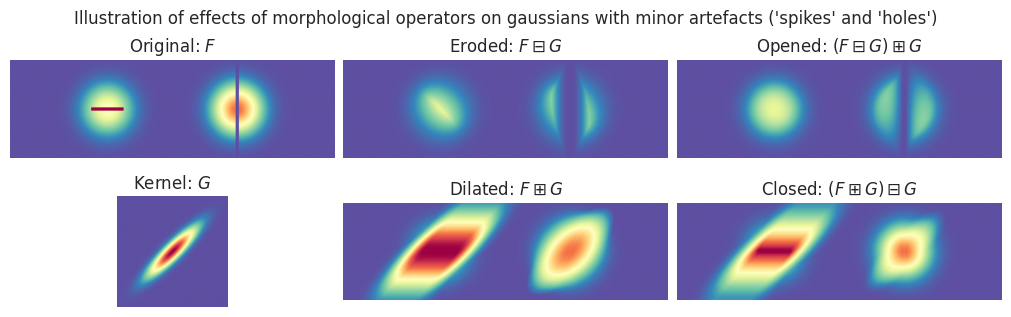
\includegraphics[width=\textwidth]{figures/closing.png}
  \caption{Illustration of the effects of opening and closing, where warmer (red) colors  indicate higher values, and colder (blue) colors  indicate lower values.}
  \label{fig:closing-illust}
\end{figure}

\section{Variations on the convolution in CNNs}
The four parameters of a convolution: stride, padding, dilation, groups. \comment{\ldots\ldots}
\section{Other nonlinear fields}
Log and root \cite{bellaardaxiomatic} \comment{\ldots\ldots}

\section{Quadratic distance functions}
In general, we may wish to weigh dimensions differently. \cite{Boomgaard1999NumericalSS} \comment{\ldots\ldots}

\newpage
\section{Learning positive definite matrices}
\label{sec:learning-pdm}
While there are many methods for parameterising a $2\times2$ positive definite matrix, since the calculation of the distance as used in the quadratic distance function is equivalent to the Mahanalobis distance, we may wish to view the matrix as a covariance matrix $\Sigma \in \mathbb{R}^{2\times2}$. Since $\Sigma$ must be symmetric, we know by the spectral theorem that $\Sigma$ is diagonalisable \cite{poole2015linear}:
\begin{align}
\textrm{For some orthogonal matrix }Q &\in \mathbb{R}^{2\times 2} \textrm{, and} \nonumber \\
\textrm{for some diagonal matrix }D &\in \mathbb{R}^{2\times 2} \textrm{,}\nonumber \\
\Sigma &= QDQ^T\\
&= Q \begin{bmatrix}
	 \sigma_1^2 & 0\\ 0 &  \sigma_2^2
\end{bmatrix} Q^T
\end{align}
Here, Q (as an orthogonal matrix) can either be a rotation  or a reflection. However, since $Q$ occurs twice, its determinant cancels, and fixing $Q$ to be a rotation does not reduce expressivity (see Appendix \ref{sec:red-mirr}). As such, we can use:
\begin{align}
\Sigma = \begin{bmatrix}
	\cos \phi & -\sin \phi \\ \sin\phi & \cos\phi
\end{bmatrix}\begin{bmatrix}
	 \sigma_1^2 & 0\\ 0 &  \sigma_2^2
\end{bmatrix} \begin{bmatrix}
	\cos \phi & \sin \phi \\ -\sin\phi & \cos\phi
\end{bmatrix}
\end{align}
This parameterisation can be efficiently inversed for the quadratic form, as \begin{align}
	\Sigma^{-1} &= (QDQ^T)^{-1}\\
	&= (Q^T)^{-1} D^{-1} Q^{-1}\\
	&= Q\begin{bmatrix}
	 \frac{1}{\sigma_1^2} & 0\\ 0 &  \frac{1}{\sigma_2^2}
\end{bmatrix}Q^T
\end{align}
In order for $\Sigma$ to be positive-definite, $\sigma_1^2$ and $\sigma_2^2$ are required to be strictly positive, while there are no constraints on $\phi$. As such, for any $\boldsymbol{\theta}\in\mathbb{R}^3$:
\begin{align}
\textrm{Let }\boldsymbol{\theta}&=\begin{bmatrix}
	\theta_1\\
	\theta_2\\
	\theta_3\\
\end{bmatrix}=\begin{bmatrix}
	\log|\sigma_1| \\
	\log|\sigma_2|\\
	\phi\\
\end{bmatrix}, \textrm{ then a valid $\Sigma^{-1}$ would be} \\
\Sigma^{-1} &= \begin{bmatrix}
	\cos \theta_3 & -\sin \theta_3 \\ \sin\theta_3 & \cos\theta_3
\end{bmatrix}\begin{bmatrix}
	 e^{-2\theta_1} & 0\\ 0 &  e^{-2\theta_2}
\end{bmatrix} \begin{bmatrix}
	\cos \theta_3 & \sin \theta_3 \\ -\sin\theta_3 & \cos\theta_3
\end{bmatrix}
\end{align}
Since we placed no assumptions on $\boldsymbol{\theta}$, it is safe for a black-box or gradient-based optimiser to adjust in any direction, as the resulting $\Sigma$ will always be a positive definite matrix.

This parameterisation has the advantage of being easily interpretable: $e^{\theta_1}$ and $e^{\theta_2}$ are the standard deviations of a hypothetical normal distribution in the first and second principal axis of the quadratic, while $\theta_3$ is the counter-clockwise angle the first principal axis forms with the x-axis. An alternative parameterisation, based on the Pearson correlation coefficient, can be found in Appendix \ref{sec:pearson}.
\chapter{Experiments}
\comment{I only really want to write the accompanying text when I have a clear idea of what the experiments are going to be: for now, I'm just putting some graphs in from the test experiments I conducted.}
\begin{figure}[h!]
	\center
  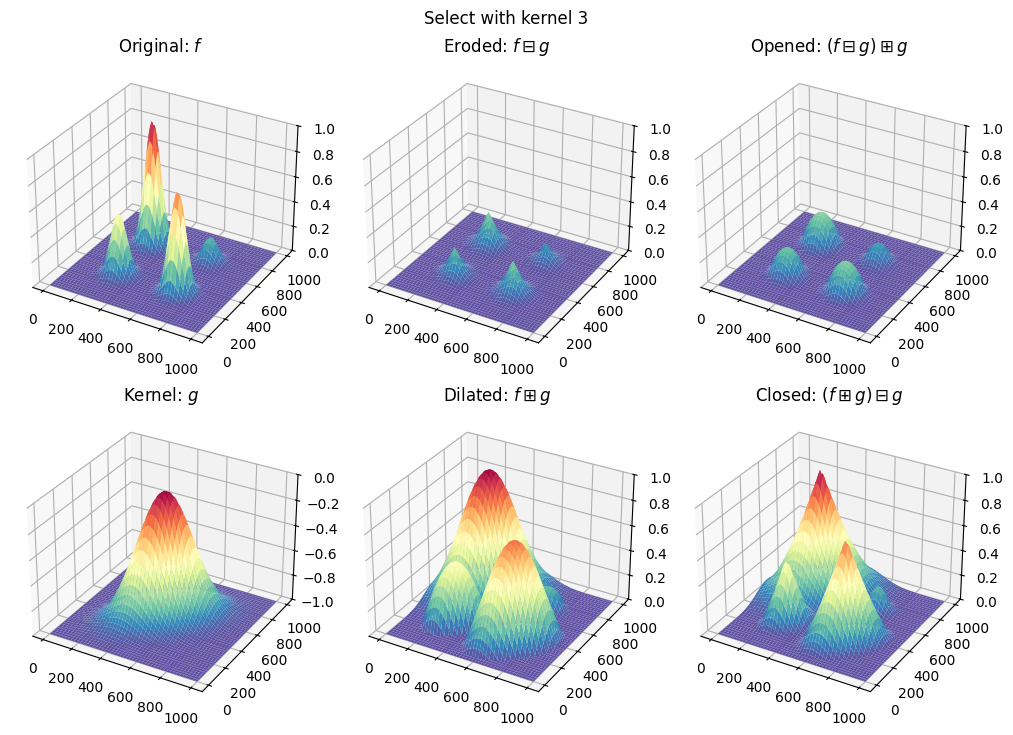
\includegraphics[width=\textwidth]{figures/morphological_3d.png}
  \caption{Illustration of the effects of dilation, erosion and their combination in two dimensions, with height representing the function value.}
  \label{fig:dil-illust}
\end{figure}
\begin{figure}[h!]
	\center
  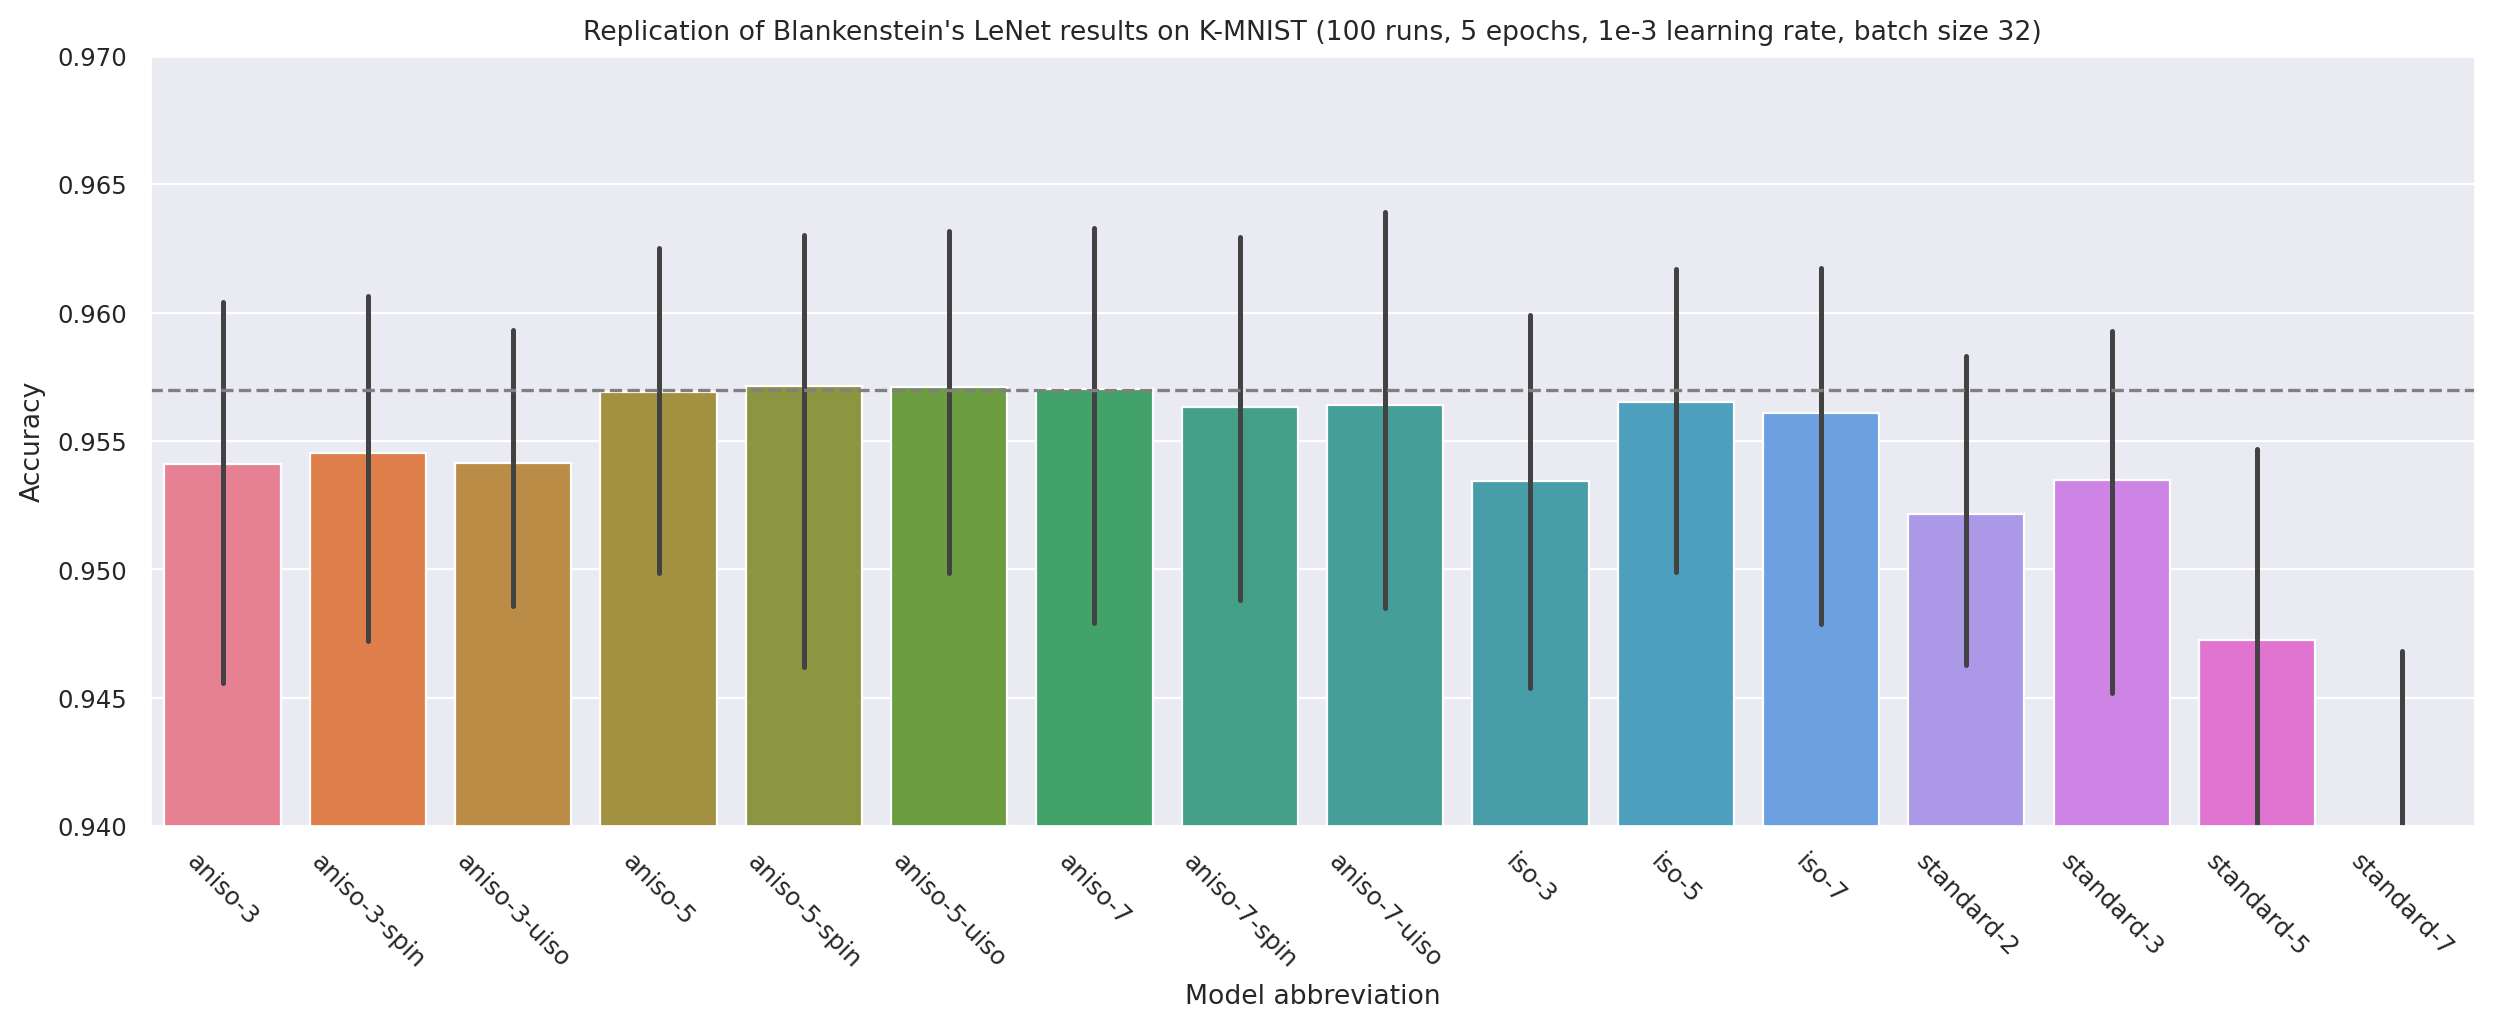
\includegraphics[width=\textwidth]{figures/thierry_replication.png}
  \caption{Replication of Blankenstein's LeNet results \cite{thierrybsc} }
  \label{fig:dil-illust}
\end{figure}
\begin{figure}[h!]
	\center
  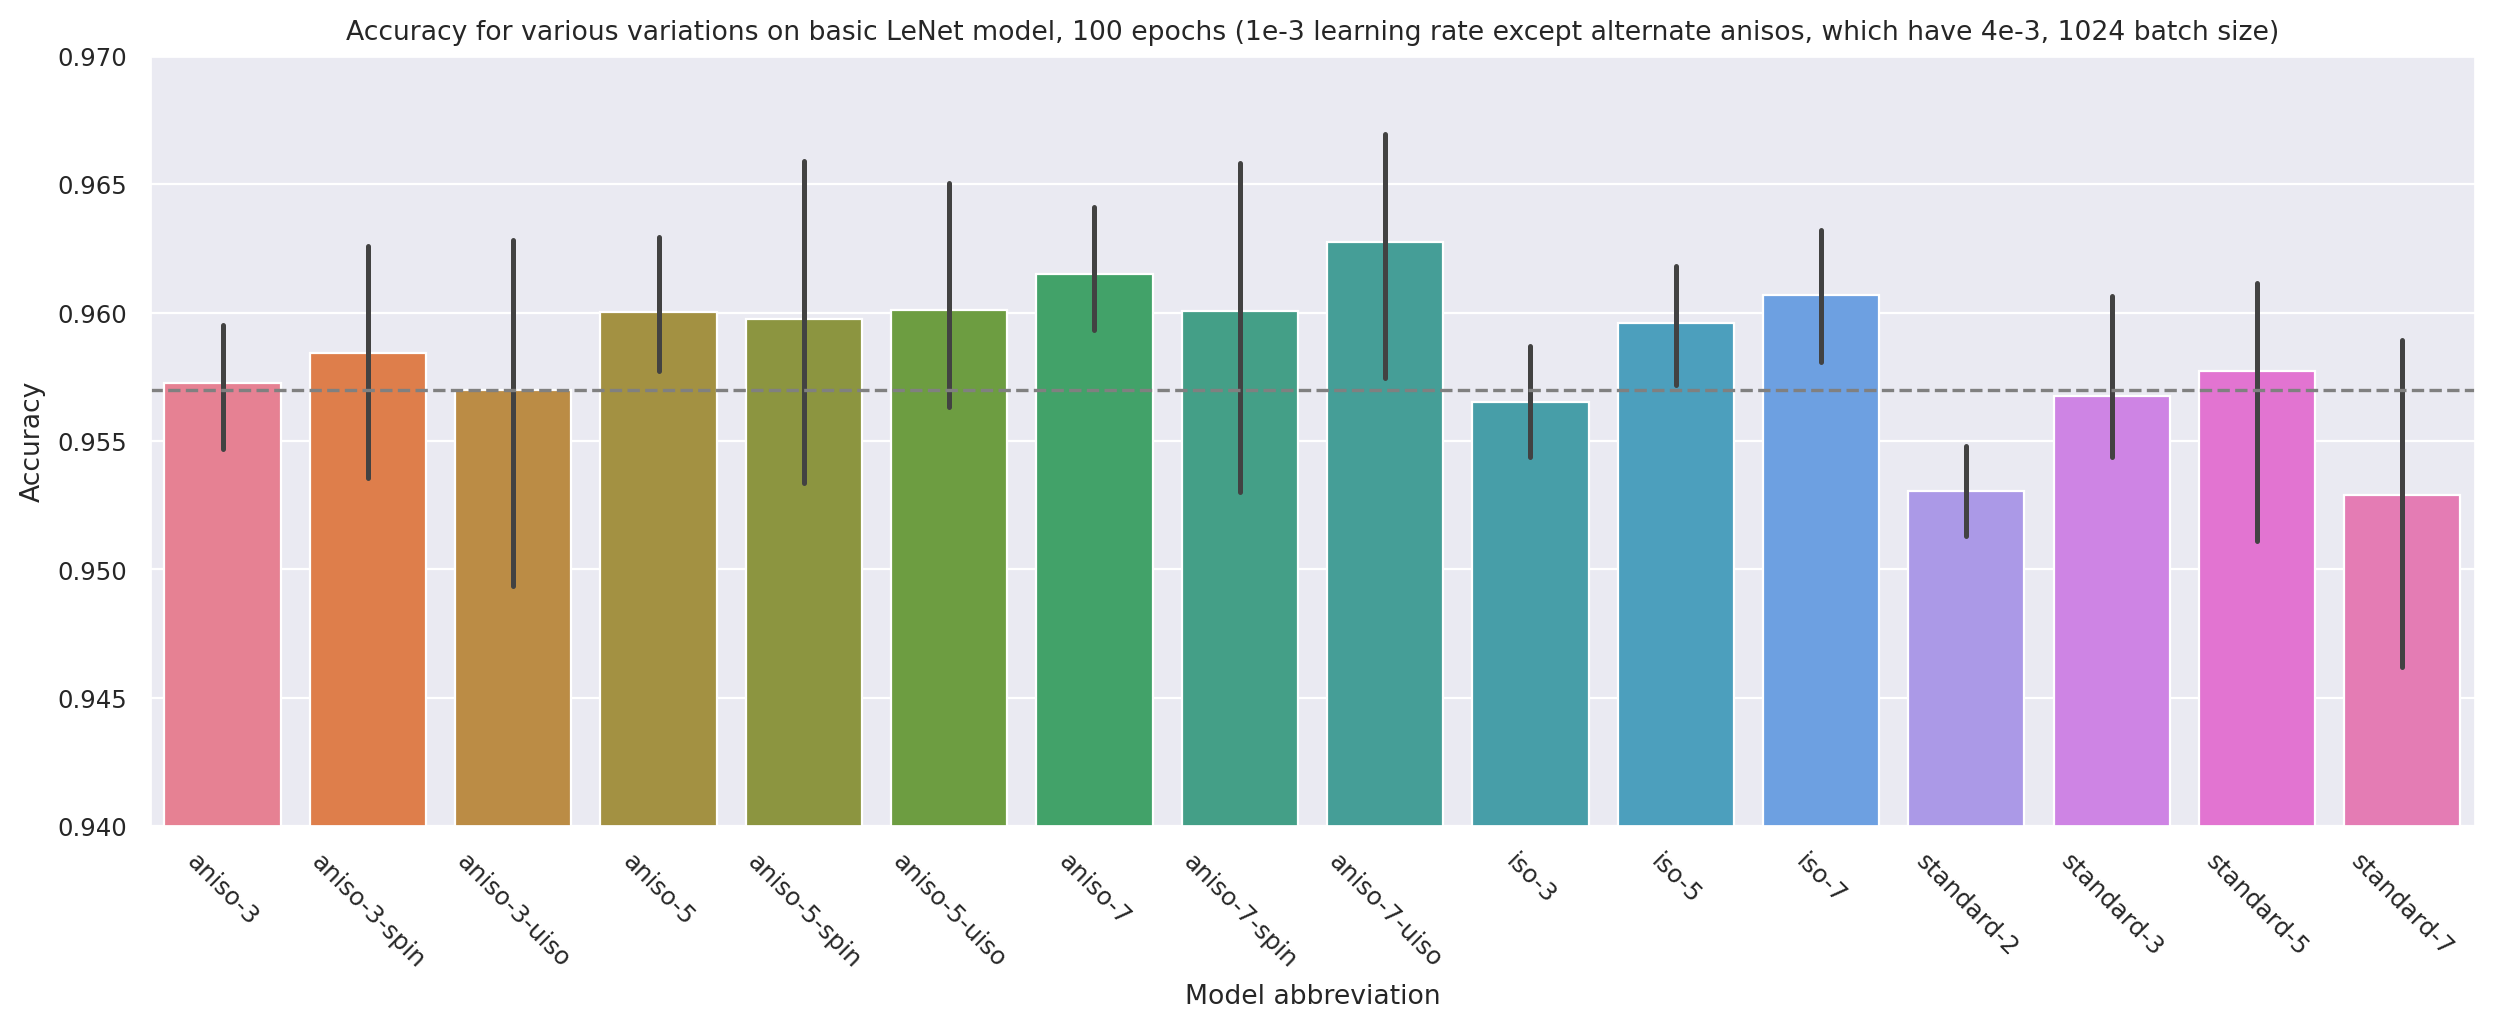
\includegraphics[width=\textwidth]{figures/100ep_extension.png}
  \caption{Extension of LeNet results using more (100) epochs, with the aniso results other than the base aniso-3/5/7 being obtained with higher LR}
  \label{fig:dil-illust}
\end{figure}


\chapter{Conclusion}
\comment{\ldots\ldots}

\bibliographystyle{ieeetr}
\bibliography{references}

\newpage
\chapter{Appendix}
\section{Redundancy of mirroring in $QDQ^T$}
\label{sec:red-mirr}
Suppose we had some symmetric $\Sigma \in \mathbb{R}^{2\times 2}$; we could then use orthogonal diagonalisation to write $\Sigma = QDQ^T$ for some orthogonal Q and diagonal D.

In \ref{sec:learning-pdm}, the claim was made that requiring $Q$ to be a rotation (and not a reflection) did not decrease the expressivity of the representation, i.e. all symmetric positive definite $\Sigma$ are representable as $RDR^T$ with R being a rotation. To show this, we can suppose some reflection $Q\in \mathbb{R}^{2\times 2}$, and see that $Q$ can be written as a rotation with angle $\phi$ ($R_\phi$) of a reflection in the x-axis \cite{poole2015linear}:
\begin{align}
	Q=\begin{bmatrix}
		\cos \phi  &  \sin \phi  \\
		\sin \phi  &  -\cos \phi
	\end{bmatrix} &= \begin{bmatrix}
		\cos \phi  &  -\sin \phi  \\
		\sin \phi  &  \cos \phi
	\end{bmatrix} \begin{bmatrix}
		1  &  0  \\
		0  &  -1
	\end{bmatrix} = R_\phi \begin{bmatrix}
		1  &  0  \\
		0  &  -1
	\end{bmatrix} \label{eq:refl-rot}
\end{align}
Then, we can write out the orthogonal diagonalisation using \ref{eq:refl-rot}:
\begin{align}
	\Sigma&=QDQ^T \\
	&= \left(R_\phi \begin{bmatrix}
		1  &  0  \\
		0  &  -1
	\end{bmatrix}\right)D\left(R_\phi \begin{bmatrix}
		1  &  0  \\
		0  &  -1
	\end{bmatrix}\right)^T \\
	&= R_\phi \begin{bmatrix}
		1  &  0  \\
		0  &  -1
	\end{bmatrix} \begin{bmatrix}
		\sigma_1^2  &  0  \\
		0  &  \sigma_2^2
	\end{bmatrix} \begin{bmatrix}
		1  &  0  \\
		0  &  -1
	\end{bmatrix} R_\phi^T \\
%	&= R_\phi \begin{bmatrix}
%		\sigma_1^2  &  0  \\
%		0  &  -\sigma_2^2
%	\end{bmatrix} \begin{bmatrix}
%		1  &  0  \\
%		0  &  -1
%	\end{bmatrix} R_\phi^T \\
	&= R_\phi \begin{bmatrix}
		\sigma_1^2  &  0  \\
		0  &  \sigma_2^2
	\end{bmatrix} R_\phi^T \\
	&= R_\phi D R_\phi^T \\&&\qed\nonumber
\end{align}
\newpage
\section{Exact dilation and erosion with clipped kernels using Lipschitz conditions on $F$}
\label{sec:lipschitz}
\comment{Todo: proof, and better name for this section}

\newpage
\section{Alternative parameterisation for $\Sigma \in \mathbb{R}^{2\times 2}$}
\label{sec:pearson}
A different way of parameterising a $2\times 2$ covariance matrix  would be to use the Pearson correlation coefficient $\rho$ instead of the angle $\phi$. 
We can then keep the covariance matrix in its Cholesky decomposed form, using a lower triangular $L$ such that $\Sigma=LL^T$. Then, for any $\boldsymbol{\theta}\in\mathbb{R}^3$, we can find the corresponding $L$:
\begin{align}
\textrm{Let }\boldsymbol{\theta}&=\begin{bmatrix}
	\theta_1\\
	\theta_2\\
	\theta_3\\
\end{bmatrix}=\begin{bmatrix}
	\log|\sigma_1| \\
	\log|\sigma_2|\\
	\tan\rho\\
\end{bmatrix}, \textrm{ then a valid $\Sigma$ would be} \\
	\Sigma &= \begin{bmatrix}
 \sigma_1^2 & \sigma_1\sigma_2\rho \\
  \sigma_1\sigma_2\rho & \sigma_2^2 \\
\end{bmatrix}
= LL^T = \begin{bmatrix}
 l_{11} & 0 \\
  l_{21} & l_{22} \\
\end{bmatrix}\begin{bmatrix}
 l_{11} & l_{21} \\
  0 & l_{22} \\
\end{bmatrix}\\
&=\begin{bmatrix}
 l_{11}^2 & l_{11}l_{21} \\
  l_{11}l_{21} & l_{21}^2 + l_{22}^2 \\
\end{bmatrix}\hspace{0.5cm}\\
\textrm{As such,}&\textrm{ we know that:}\nonumber\\
	l_{11} &= \sqrt{\sigma_1^2} =\sigma_1=\exp(\theta_1)\\
	l_{21} &= \frac{\sigma_1\sigma_2\rho}{\sigma_1}=\sigma_2\rho=\exp(\theta_2)\tanh(\theta_3) \\
%	l_{21}^2 + l_{22}^2 &= \sigma_2^2 \textrm{, so}\\
	l_{22} &= \sqrt{\sigma_2^2 - \sigma_2\rho} = \sqrt{\exp(2\theta_2)-\exp(\theta_2)\tanh(\theta_3)}
\end{align}
which is then a valid parameterisation for the Cholesky decomposed form for a $2\times 2$ positive definite matrix\footnote{To extend this parameterisation for higher dimensions, see the  Cholesky-Banachiewicz algorithm for the Cholesky decomposition}. If we keep the covariance matrix in this triangular form, we can see that the quadratic form can be calculated in an efficient manner:

(based on the PyTorch code for the multivariate normal PDF)
\begin{align}
	\mathbf{x}^T\Sigma^{-1}\mathbf{x}
	&= \mathbf{x}^T(LL^T)^{-1}\mathbf{x}\\
	&= \mathbf{x}^T(L^T)^{-1}L^{-1}\mathbf{x}\\
	&= \mathbf{x}^T(L^{-1})^{T}L^{-1}\mathbf{x}\\
	&= ((L^{-1})\mathbf{x})^T(L^{-1}\mathbf{x})\\
	&= (L^{-1}\mathbf{x})\cdot(L^{-1}\mathbf{x})\\
\textrm{Suppose }\mathbf{b}&=L^{-1}\mathbf{x}, \textrm{ then} \nonumber\\
	L\mathbf{b}&=\mathbf{x}, \textrm{ so}\nonumber\\
	\mathbf{b}&= \textsc{solve-triangular}(L, \mathbf{x})\\
	\mathbf{x}^T\Sigma^{-1}\mathbf{x} &= \mathbf{b}\cdot\mathbf{b}
\end{align}
where $\textsc{solve-triangular}$ performs efficient backsubstitution to avoid computing the inverse. This method is significantly (>5x) faster on the CPU it was tested on while still showing modest performance improvements on the GPU it was tested on ($\sim 10\%$). However, interpretation of the Pearson correlation coefficient may be more challenging compared to interpreting the angular offset of the first primary axis, and the calculation of the quadratic forms is a negligible part of the model runtime on the GPU, so it was chosen to instead parameterise $\Sigma$ with the angle $\phi$.


\end{document}
